\PassOptionsToPackage{
  unicode,
  pdfusetitle,
  colorlinks,
  linkcolor=vertexDarkRed,
  urlcolor=vertexDarkRed,
  citecolor=vertexDarkRed,
}{hyperref}
\documentclass[
  aspectratio=1610,
]{beamer}
\usetheme{vertex}
\usepackage[american]{babel}

\usepackage[autostyle]{csquotes}

\usepackage{fontspec}
\usepackage{fontawesome5}
\usepackage{graphicx}

\usepackage{tabu}

\usepackage[outputdir=build]{minted}
\usepackage{xcolor}
\usepackage{xparse}
\usepackage{tcolorbox}
\tcbuselibrary{minted}
\tcbuselibrary{skins}
\tcbuselibrary{xparse}
\usepackage{accsupp}

\usepackage{tikz}
\usetikzlibrary{
  graphs, arrows, positioning, graphdrawing
}

\usepackage{bookmark}
\usepackage[shortcuts]{extdash}


\definecolor{positive}{HTML}{15B01A}
\colorlet{negative}{vertexDarkRed}
\setmonofont{Fira Mono}

\newcommand\headline[1]{\textbf{\Large\strut{}#1}\newline}
\newcommand\headlineframe[1]{%
  \begin{frame}[c]%
    \begin{center}%
      \Huge\color{vertexDarkRed}#1%
    \end{center}%
  \end{frame}%
}%

\renewcommand\theFancyVerbLine{%
  \BeginAccSupp{method=escape,ActualText={}}%
  {\ttfamily\tiny\arabic{FancyVerbLine}}%
  \EndAccSupp{}%
}%

\tcbset{codebox/.style={
  listing engine=minted,
  colback=black!5!white,
  colframe=vertexDarkGrey,
  listing only,
  left=5mm,
  top=2pt,
  bottom=0pt,
  boxsep=3pt,
  enhanced,
  overlay={%
    \begin{tcbclipinterior}
      \fill[black!20!white] (frame.south west) rectangle ([xshift=5mm]frame.north west);
    \end{tcbclipinterior}
  },
}}

\DeclareTCBInputListing{inputcode} {O{} m m O{}} {
  codebox,
  listing file=#2,
  minted language=#3,
  minted options={
    fontsize=\footnotesize,
    breaklines,
    autogobble,
    linenos,
    numbersep=3mm,
    #4
  },
  #1
}
\DeclareTCBListing{code} {O{} m} {
  codebox,
  minted language=#2,
  minted options={
    fontsize=\footnotesize,
    breaklines,
    autogobble,
    linenos,
    numbersep=3mm
  },
  #1
}

\newcommand\copywarning{%
  \begin{frame}[c]{Warning}%
    \centering%
    \Large\color{vertexDarkRed}%
    \vspace{3\baselineskip}

    \begin{columns}[onlytextwidth, c]%
      \begin{column}{0.15\textwidth}%
        \fontsize{60}{60}\selectfont%
        \faIcon{biohazard}%
      \end{column}%
      \hfill%
      \begin{column}{0.7\textwidth}%
        \centering
        Copying commands or code from PDF files is\\ \textbf{dangerous}
      \end{column}%
      \hfill%
      \begin{column}{0.15\textwidth}%
        \hfill%
        \fontsize{60}{60}\selectfont%
        \hfill\faIcon{radiation}%
      \end{column}%
    \end{columns}%

    \vspace{2\baselineskip}
    Copy from the example files in the repository or type by hand.

    \bigskip
    Typing by hand is best for learning.
  \end{frame}
}


\tikzset{
  invisible/.style={opacity=0,text opacity=0},
  visible on/.style={alt={#1{}{invisible}}},
  alt/.code args={<#1>#2#3}{%
    \alt<#1>{\pgfkeysalso{#2}}{\pgfkeysalso{#3}} % \pgfkeysalso doesn't change the path
  },
}


\author[M. Nöthe]{Maximilian Nöthe}
\title[VC with Git]{Version Control using \texttt{git}}
\date[2021-06-08]{%
  \raisebox{-1.5cm}{
\includegraphics[height=3cm]{../logo-Escape_cropped.png}}
  \Large Summer School – 2021-06-08
}
\institute[TU Dortmund]{Astroparticle Physics, TU Dortmund}

\begin{document}

\maketitle

\begin{frame}[c]{Overview}
\tableofcontents
\end{frame}

\section{whoami}
\begin{frame}[c, fragile]{\texttt{whoami}}
  \begin{columns}[onlytextwidth, T]%
    \begin{column}{0.8\textwidth}%
      \begin{itemize}
        \item[{\Large\faGithub}] \href{https://github.com/maxnoe}{maxnoe}
        \item[{\Large\faUniversity}] PostDoc @ TU Dortmund
        \item[{\Large\faGraduationCap}] PhD in astroparticle physics, also @ TU Dortmund
        \item[{\Large\faFlask}] Gamma-ray astronomy with Imaging Atmospheric Cherenkov Telescopes (CTA, FACT, MAGIC)
        \item[{\Large\faMicroscope}] Data Analysis, Statistics, Machine Learning, Software Development
        \item[{\Large\faLaptopCode}] \faPython, C++, \LaTeX{}, (neo)vim, zsh, astropy, matplotlib, ...
        \item[{\Large\faHeart}] FOSS, Open Science, Best Practices
      \end{itemize}
    \end{column}%
    \hfill%
    \begin{column}{0.19\textwidth}%
      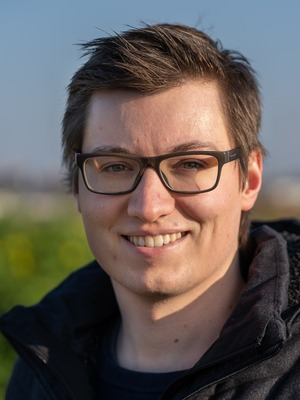
\includegraphics[height=\textwidth]{images/max.jpg}
    \end{column}%
  \end{columns}%
\end{frame}

\copywarning{}

\section[Version Control]{What is version control and why do we need it?}

\begin{frame}[c]%
  \begin{center}%
    \Huge\color{vertexDarkRed}What is version control and why do we need it?%
  \end{center}%
\end{frame}%


\begin{frame}[c]{What is Version Control?}
  \begin{itemize}
    \item Version Control tracks changes of a (collection of) document(s)
    \item This can basically be anything:
      \begin{itemize}
        \item software
        \item legal documents
        \item documentation
        \item scientific paper
        \item images
        \item ...
      \end{itemize}
    \item We will call a snapshot of such a collection a \enquote{revision}.
    \item Revisions are the complete history of our projects
  \end{itemize}
\end{frame}

\begin{frame}[c]{Why Use Version Control?}
  \begin{itemize}
    \item Allows us to go back to arbitrary revisions
    \item Shows differences between revisions
    \item Enables collaborative working
    \item Acts as backup
  \end{itemize}
\end{frame}

\begin{frame}[c]{Why Use Version Control?}
  Most Version Control Systems (VCS) make answering the following questions easy:
  \begin{description}
    \item[What?] What changed from revision \emph{a} to revision \emph{b}?
    \item[Who?] Who made a change? Who contributed?
    \item[Why?] VCS usually encourage or even force adding explanations to changes.
    \item[When?] In which revision was a bug introduced or fixed?
  \end{description}

  \onslide<2>{%
    \begin{center}
      \Large\textcolor{vertexDarkRed}{Version Control is a basic requirement for reproducible science}  
    \end{center}
  }
\end{frame}

\section{Git}
\headlineframe{
    
\includegraphics[width=0.7\textwidth]{logos/git.pdf}
}
\begin{frame}[c]
    \begin{columns}[onlytextwidth, c]%
      \begin{column}{0.3\textwidth}%
        \includegraphics[width=\textwidth]{build/figures/xkcd_git.png}\\%
        \small \href{https://xkcd.com/1597/}{R. Munroe, xkcd.com/1597}
      \end{column}%
      \hfill%
      \begin{column}{0.695\textwidth}%
        \begin{itemize}
          \item Created by Linus Torvalds in 2005 for the \href{https://github.com/torvalds/linux}{Linux Kernel}
          \item Most widely used VCS in FOSS
          \item Distributed, allows offline usage
          \item Much better branching model than precursors like SVN
        \end{itemize}
      \end{column}%
    \end{columns}%
\end{frame}

\headlineframe{The Git Repository}
\begin{frame}{Central Concept: Repository}
  \begin{itemize}
    \item \texttt{git init} creates a git repository in the current working directory
    \item All git data is stored in the \texttt{.git} directory.
    \item Git has three different areas, data can reside in:
  \end{itemize}

  \centering
  \begin{tikzpicture}[
      line width=1.5,
      gitstep/.style={
        draw,
        rounded corners,
        thick,
        minimum width=4cm,
        minimum height=1.2cm,
      },
    ]
    \node (wd) at (0, 0) [gitstep, fill=red!20, visible on=<1->] {Working directory};
    \node (idx) [gitstep, fill=yellow!20, below=0.4cm of wd] {Staging};
    \node (hist) [gitstep, fill=green!20, below=0.4cm of idx] {History};
    \node [right=1cm of wd, text width=0.5\textwidth, align=flush left] {
      What actually is on disk in the current working directory. 
    };
    \node [right=1cm of idx, text width=0.5\textwidth, align=flush left] {
      Changes that are saved to go into the next commit.
    };
    \node [right=1cm of hist, text width=0.5\textwidth, align=flush left] {
      The history of the project. All changes ever made. A \emph{Directed Acyclic Graph} of commits.
    };
  \end{tikzpicture}
\end{frame}

\begin{frame}{Central Concept: Repository}

  \vspace{3em}
  \centering
  \begin{tikzpicture}[
      line width=1.5,
      gitstep/.style={
        draw,
        rounded corners,
        thick,
        minimum width=4cm,
        minimum height=1.2cm,
      },
    ]
    \node (wd) at (0, 0) [gitstep, fill=red!20, visible on=<1->] {Working directory};
    \node (idx) [gitstep, fill=yellow!20, visible on=<1->, below=0.4cm of wd] {Staging};
    \node (hist) [gitstep, fill=green!20, visible on=<1->, below=0.4cm of idx] {History};
    \draw[thick,->, visible on=<2->] (wd.east) to[out=0,in=0] node[right] {\texttt{git add}} (idx.east);
    \draw[thick,->, visible on=<3->] (idx.west) to[out=180,in=180] node[left] {\texttt{git commit}} (hist.west);
  \end{tikzpicture}
\end{frame}


\begin{frame}{History}
  \only<1-2>{
    \begin{tikzpicture}
      \graph [
        grow right=1.5cm,
        nodes={
          blue!70!black,
          node font=\ttfamily,
        },
      ]{
        "v1.0.0" [visible on=<4->, green!60!black, x=6];
        a <- b <- c <- d <- main [vertexDarkRed];
        c <-[visible on=<2>] "\strut e"[x=4.5, visible on=<2>] <-[visible on=<2>] foo [vertexDarkRed, visible on=<2>, x=4.1];
      };
    \end{tikzpicture}
  }
  \only<3->{
    \begin{tikzpicture}
      \graph [
        grow right=1.5cm,
        nodes={
          blue!70!black,
          node font=\ttfamily,
        },
      ]{
        "v1.0.0" [visible on=<4->, green!60!black, x=6],
        "\strut a" <- b <- c <- {
          d <- f,
          "\strut e",
        } <- g [x=0] <- h <- {i <-[visible on=<2->] main [vertexDarkRed, visible on=<3->]};
        "v1.0.0" ->[visible on=<4->] f;
      };
    \end{tikzpicture}
  }

  \begin{itemize}
    \item<1-> \textcolor{blue}{Commit}: State/Content at a given time
      \begin{itemize}
        \item Contains a commit message to describe the changes
        \item Always points to its parent(s)
        \item Is identified by a hash of the content, message, author, parent(s), time
      \end{itemize}
    \item<2-> \textcolor{vertexDarkRed}{Branch}: A named pointer to a commit
      \begin{itemize}
        \item Development branches
        \item Default branch: \texttt{master} or \texttt{main}
        \item Moves to the next child if a commit is added
      \end{itemize}
    \item<4-> \textcolor{green!60!black}{Tag}: Fixed, named pointer to a commit
      \begin{itemize}
        \item For important revisions, e.g. release versions or version used for a certain paper
      \end{itemize}
  \end{itemize}
\end{frame}

\begin{frame}[fragile]{Initial Setup}
  \begin{itemize}
    \item The first thing you should do after installing git is tell it who you are:
      \begin{code}[title={\textcolor{negative!60!white}{\faExclamationTriangle} Fill your own information! \textcolor{negative!60!white}{\faExclamationTriangle}}]{bash}
        $ git config --global user.name "Maximilian Nöthe"
        $ git config --global user.email "maximilian.noethe@tu-dortmund.de"
      \end{code}
    \item This information is required as it will be added to each commit you make
    \item Hosting providers map commits to users by the commit email
  \end{itemize}
\end{frame}

\begin{frame}[fragile]{Creating or Cloning a Repository}
  \begin{itemize}
    \item Create a new git repository in the current directory
      \begin{code}{bash}
        $ git init
      \end{code}
    \item Clone (download) a repository from a server, e.\,g.\ GitHub
      \begin{code}{bash}
        $ git clone <url>
      \end{code}
    \item Remove all traces of git from a repository
      \begin{code}{bash}
        $ rm -rf .git
      \end{code}
      \textcolor{negative}{\faExclamationTriangle} This is not recoverable locally \textcolor{negative}{\faExclamationTriangle}
  \end{itemize}
\end{frame}

\begin{frame}[fragile]{\texttt{git status}}
  \begin{itemize}
    \item Shows current branch and new, modified, added files
    \item Make a habit of calling \mintinline{text}+git status+ often
    \item Concise version with \mintinline{text}+git status -s+
  \end{itemize}
\end{frame}

\begin{frame}{\texttt{git add}, \texttt{git mv}, \texttt{git rm}, \texttt{git reset}}
  \begin{tabu}{>{\ttfamily}l X[,L]}
    git add <file> … & Add files to the staging \\
    git mv           & like \texttt{mv}, stages automatically \\
    git rm           & like \texttt{rm}, stages automatically \\
    git reset <file> & Removes changes/files from the staging area
  \end{tabu}
\end{frame}

\begin{frame}[fragile]{Creating a new commit}
  \begin{itemize}
    \item Create a new commit from the changes in the staging area.\\
      This will open editor for the commit message, most likely \emph{vim}\\
      \begin{code}{bash}
        $ git commit
      \end{code}
    \item You can also give the message directly on the command line:
      \begin{code}{bash}
        $ git commit -m "Fix critical bug in flight control system"
      \end{code}
    \item If you are not familiar with vim, you might want to change the editor. \\
      The exact settings depend on the editor, to use VS Code or nano:
      \begin{code}{bash}
        $ git config --global core.editor "code --wait"
        $ git config --global core.editor nano
      \end{code}
  \end{itemize}
\end{frame}

\begin{frame}[fragile]{What is a good commit?}
  \begin{itemize}
    \item Commits should be small, logical units
    \item \enquote{Commit early, commit often}
    \item It is common convention to formulate the commit subject as imperative:\\
      \begin{center}
        \texttt{Change value of foo to 6}
      \end{center}
    \item Style guide for commit messages:
      \begin{code}{text}
        Subject line, short description, best < 60 characters

        After one empty line, a detailed description of the commit.
        Explain why the change was necessary and give details.
        * Use bullet point lists for stuff
        * Link releveant issues, #2

        Give credit to other people when working together:
        Co-authored-by: Thomas Vuillaume <thomas.vuillaume@lapp.in2p3.fr>
      \end{code}
  \end{itemize}
\end{frame}

\begin{frame}[c, fragile]{Accessing the log}
  \begin{itemize}
    \item Shows author information, date, hash, message
      \begin{code}{bash}
        $ git log
      \end{code}
    \item Supports ranges:
      \begin{code}{bash}
        $ git log <a>..<b>
      \end{code}
      (All commits reachable from \texttt{<b>} but not from \texttt{<a>})
    \item More concise log, helpful for use with \texttt{grep} \\
      \begin{code}{bash}
        $ git log --oneline
      \end{code}
    \item Showing branches in \enquote{ASCII art}: \\
      \begin{code}{bash}
        $ git log --all --decorate --graph
      \end{code}
  \end{itemize}
\end{frame}

\begin{frame}[fragile]{\texttt{git diff}}
  Shows the differences between versions.

  \begin{itemize}
    \item Show diff between the current working directory and the staging area:
      \begin{code}{bash}
        $ git diff
      \end{code}

    \item Show diff between the staging area and the last commit: \\
      \begin{code}{bash}
        $ git diff --staged
      \end{code}
      This is \emph{very} useful, since this will become be the next commit. \\
      Run before \mintinline{bash}+git commit+ and check for mistakes.
    \item Show diff between two files, commits, branches, ...
      \begin{code}{bash}
        $ git diff <arg1> <arg2>
      \end{code}
  \end{itemize}
\end{frame}

\begin{frame}[fragile]{Loading commits / restoring files}
  \begin{itemize}
    \item Load a certain commit from the history into the CWD (check with \texttt{git log}) \\
      \begin{code}{bash}
        $ git checkout <commit>
      \end{code}
    \item Restore a file to the version from the last commit (throwing any changes away)
      \begin{code}{bash}
        git restore <file>
      \end{code}
    \item Restore a file to a version from a specific commit or branch
      \begin{code}{bash}
        git restore --source=<source> <file>
      \end{code}
  \end{itemize}
  \begin{tabu}{>{\ttfamily}l X[,L]}
  \end{tabu}
\end{frame}

\begin{frame}[c, fragile]{Note on older versions of git}
  \begin{itemize}
    \item In older versions of git, \mintinline{bash}+git checkout+ had many different tasks, which is confusing
      \begin{itemize}
        \item Loading commits into the working directory
        \item Restoring files to another version
        \item Switching branches
      \end{itemize}
    \item Recent versions of git added \mintinline{bash}+git restore+ for restoring files
    \item Iff you have an old version of git and cannot upgrade easily, use
      \begin{code}{bash}
        $ git checkout <source> -- <file>
      \end{code}
  \end{itemize}
\end{frame}

\begin{frame}{Remotes}
  Remotes are central places, e.\,g.\ servers, where repositories can be saved and which can be used to synchronize between different clients.
  \begin{center}
  \begin{tikzpicture}[line width=1.5]
    \node (hist) [draw,rounded corners,thick,minimum width=4cm,minimum height=1.2cm,fill=green!20] {History};
    \node (remote) [below=0.4cm of hist,draw,rounded corners,thick,minimum width=4cm,minimum height=1.2cm,fill=blue!20] {Remote};
    \draw[thick,->] (hist.east) to[out=0,in=0] node[right] {\texttt{git push}} (remote.east);
    \draw[thick,->] (remote.west) to[out=180,in=180] node[left] {\texttt{git fetch}} (hist.west);
  \end{tikzpicture}
  \end{center}
\end{frame}

\begin{frame}[fragile]{Syncing with remotes}
  \begin{itemize}
    \item Download (clone) a repository from a remote
      \begin{code}{bash}
        $ git clone <url>
      \end{code}
    \item Add a new remote to the repository
      \begin{code}{bash}
        $ git remote add <name> <url>
      \end{code}
      \begin{itemize}
        \item The default remote is called \enquote{origin} by convention
        \item When you clone a repository, the \enquote{origin} remote will already be setup
      \end{itemize}
    \item Download changes from the default or a specific remote:
      \begin{code}{bash}
        $ git fetch [remote]
      \end{code}
    \item Download changes from the default remote and merge them into your local branch
      \begin{code}{bash}
        $ git pull
      \end{code}
  \end{itemize}
\end{frame}

\begin{frame}[fragile]{Syncing with remotes}
  \begin{itemize}
    \item Upload your current branch to its default remote
      \begin{code}{bash}
        $ git push
      \end{code}
    \item Set the default remote for branch and push (needed when pushing a new branch for the first time)
      \begin{code}{bash}
        $ git push -u origin branch
      \end{code}
  \end{itemize}
\end{frame}


\begin{frame}{Typical single-branch workflow}
  \begin{enumerate}
    \item[0.] Get / create / update the repository
      \begin{description}[if exists]
        \item[If new] Create or clone repository : \texttt{git init}, \texttt{git clone <url>}
        \item[If exists] \texttt{git pull}
      \end{description}
    \item Work
      \begin{enumerate}
        \item Edit files and build/test
        \item Add changes to the next commit: \texttt{git add}
        \item Save added changes in the history as \emph{commit}: \texttt{git commit}
      \end{enumerate}
    \item Download commits that happend in the meantime: \texttt{git pull}
    \item Upload your own: \texttt{git push}
    \item Go back to 1
  \end{enumerate}
\end{frame}


\begin{frame}[c]{Working using multiple branches – GitHub Workflow}
  There are multiple models of working together with git using branches

  Simplest and most popular: \enquote{GitHub-Workflow}

  \begin{itemize}
    \item Nobody directly commits into the main branch
    \item A new branch is created for each new feature / change / bug-fix
    \item Branches should be rather short-lived
    \item Merge into the main branch as soon as possible, then delete the feature branch
    \item The main branch should always contain a working version
  \end{itemize}


  \bigskip
  \small
  Note: this workflow is only named after GitHub, you can and should also use it on
  GitLab or whatever other platform you are using.
\end{frame}

\begin{frame}[fragile]{Branches}
  \begin{itemize}
    \item Create a new branch pointing to the current commit
      \begin{code}{bash}
        $ git branch <name>
      \end{code}
    \item Switch to branch \texttt{<name>}
      \begin{code}{bash}
        $ git switch <name>
      \end{code}
    \item Create a new branch and change to it
      \begin{code}{bash}
        $ git switch -c <name>
      \end{code}
    \item Merge the changes of branch \texttt{<other>} into the current branch
      \begin{code}{bash}
        $ git merge <other>
      \end{code}
  \end{itemize}

  \smallskip
  \small Note: As with \mintinline{bash}+git restore+, \mintinline{bash}+git switch+ is a relatively new addition to git. 
  Use \mintinline{bash}+git checkout [-b] <branch>+ for older versions
\end{frame}

\begin{frame}[c, fragile]{Default branch name}

  \begin{itemize}
    \item Recently, a political correctness discussion happened around  master/slave terminology in tech
    \item Many software projects have since replaced those terms
    \item While not directly related to master/slave, git also enabled to change the name of the default branch
    \item GitHub and GitLab now use \texttt{main} as default for new repositories
    \item Currently, you will encounter both \texttt{master} and \texttt{main}
    \item Use \texttt{main} locally (when using \mintinline{bash}+git init+)
      \begin{code}{bash}
      $ git config --global init.defaultBranch main
      \end{code}
  \end{itemize}

\end{frame}

\begin{frame}[fragile]{Beware: Merge conflicts}
  Happens when git can't merge automatically, e.\,g.\ two people edited the same line.

  \begin{enumerate}
    \item Open the files with conflicts
    \item Find the lines with conflicts and resolve by manually editing them
      \begin{code}{text}
        <<<<<<< HEAD
        foo
        ||||||| merged common ancestors
        bar
        =======
        baz
        >>>>>>> Commit-Message
      \end{code}
    \item Commit merged changes:
      \begin{code}{bash}
        $ git add …
        $ git commit
      \end{code}
  \end{enumerate}
  useful: \texttt{git config --global merge.conflictstyle diff3}
\end{frame}

\begin{frame}[t]{Relevant XKCD}%
  \centering%
  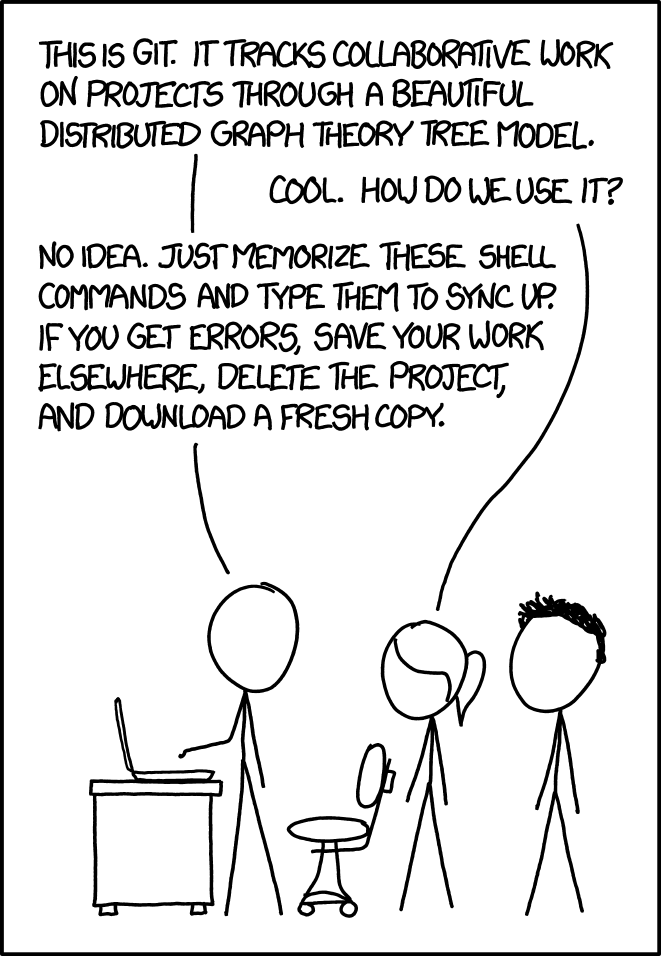
\includegraphics[height=0.95\textheight]{images/xkcd.png}%
  \href{https://xkcd.com/1597}{R.~Munroe, xkcd.com/1597}%
\end{frame}

\begin{frame}[fragile]{\texttt{.gitignore}}
  \begin{itemize}
    \item Many files or filetypes should not be put under version control
      \begin{itemize}
        \item Compilation results
        \item Files reproducibly created by scripts
        \item Config files containing credentials
        \item ...
      \end{itemize}
    \item Solution: \texttt{.gitignore} in the base of a repository
    \item One file or glob pattern per line for files that git should ignore
    \item Hosting providers have default \texttt{.gitignore} for most programming languages: \href{https://github.com/github/gitignore}{github.com/github/gitignore}
  \end{itemize}
  \begin{code}[title=Example \texttt{.gitignore}]{text}
    build/
    *.so
    __pycache__/
  \end{code}
\end{frame}

\begin{frame}[fragile]{Global \texttt{.gitignore}}
  \begin{itemize}
    \item Some files should be ignored globally for all repositories of a user
      \begin{itemize}
        \item OS specific files
        \item Editor / tool specific files
        \item ...
      \end{itemize}
    \item \mintinline{bash}+git config --global core.excludesfile $HOME/.gitignore+
  \end{itemize}

  \begin{code}[title=\mintinline{text}+$HOME/.gitignore+]{text}
    __MACOSX    # weird mac directory
    .DS_STORE   # mac finder metadata file
    *.swp       # vim backup files
    *~          # nano / gedit / emacs backup files
    desktop.ini # Windows explorer metadata file
  \end{code}
\end{frame}


\begin{frame}[c]{Some Limitations of git}
  \begin{itemize}
    \item Git is only designed to work well with text files
    \item In general, git does not handle binary files well, this includes:
      \begin{itemize}
        \item Images
        \item Document formats like odp, docx, pdf, ...
        \item Binary data files
      \end{itemize}
    \item Git cannot efficiently store these files in the history
    \item Repository size will grow quickly when often changing binary files
    \item Although being text (JSON), jupyter notebooks are also hard to use well with git
      \begin{itemize}
        \item Graphics embedded into the notebook
        \item Merge conflict resolution hard to get right
        \item Diffs not really telling what changed
        \item Tooling to improve this: nbdime, reviewnb
        \item Recommendation: only commit notebooks after running \enquote{Clear all outputs}
      \end{itemize}
  \end{itemize}  
\end{frame}

\begin{frame}[fragile]{Most common commands}
  \centering
  \begin{tikzpicture}[
      line width=1.5,
      gitstep/.style={
        draw,
        rounded corners,
        thick,
        minimum width=4cm,
        minimum height=1.2cm,
      },
    ]
    \node (wd) at (0, 0) [gitstep, fill=red!20, visible on=<1->] {Working directory};
    \node (idx) [gitstep, fill=yellow!20, visible on=<1->, below=0.4cm of wd] {Staging};
    \node (hist) [gitstep, fill=green!20, visible on=<1->, below=0.4cm of idx] {History};
    \node (remote) [below=0.4cm of hist,draw,rounded corners,thick,minimum width=4cm,minimum height=1.2cm,fill=blue!20] {Remote};

    \draw[thick,<-] ([yshift=-0.15cm] wd.east) to[out=0,in=0] node[right] {\texttt{git reset}} (idx.east);
    \draw[thick,->] ([yshift=-0.15cm] idx.west) to[out=180,in=180] node[left] {\texttt{git commit}} ([yshift=0.15cm]hist.west);

    \draw[thick,->, text width=12em] ([yshift=0.15cm] hist.east) to[out=0, in=0, looseness=3.2] node[right]{\texttt{%
      git restore\\
      git switch\\
      git checkout
    }} ([yshift=0.15cm]wd.east);
    \draw[thick,<-] ([yshift=0.15cm] idx.west) to[out=180, in=180] node[left]{\texttt{git add}} (wd.west);

    \draw[thick,<-] ([yshift=-0.15cm] hist.east) to[out=0,in=0] node[right] {\texttt{git fetch}} (remote.east);
    \draw[thick,<-] (remote.west) to[out=180,in=180] node[left] {\texttt{git push}} ([yshift=-0.15cm]hist.west);
  \end{tikzpicture}

  \mintinline{text}+git pull = git fetch && git merge <default remote>/<branch>+
\end{frame}

\headlineframe{Questions?}

\section{Git Hosting Providers}
\headlineframe{Git Hosting Providers}

\begin{frame}[c]{Git Hosting Providers}
  \begin{itemize}
    \item Several Providers and self-hosted server solutions are available
    \item Usually provide much more than just hosting the repositories
      \begin{itemize}
        \item Issue tracking
        \item Code review using pull requests
        \item Wiki
        \item Project Management, e.g. Canban boards
        \item Continuous integration
        \item Releases
      \end{itemize}
  \end{itemize}
\end{frame}

\begin{frame}[c]{Git Hosting Providers}
  \small
  \begin{tabu}{@{} X[,C] @{} X[,C] @{} X[,C] @{}}
    \href{https://github.com}{\includegraphics[width=0.75\linewidth]{figures/github.png}} &
    \href{https://gitlab.com}{\includegraphics[width=0.75\linewidth]{figures/gitlab.png}} &
    \href{https://bitbucket.org}{\includegraphics[width=0.75\linewidth]{figures/bitbucket.png}} \\
    \begin{itemize}
      \item Largest Hoster
      \item Many Open Source Projects, e.g. Python
      \item Unlimited private repositories
      \item Free CI service for public repositories
      \item Github Pro free for students / teachers / researchers
    \end{itemize}
    &
    \begin{itemize}
      \item open-source community edition
      \item paid enterprise edition with more features
      \item unlimited private repositories
      \item Self hosted or as service at \href{https://gitlab.com}{gitlab.com}
    \end{itemize}
    &
    \begin{itemize}
      \item Unlimited private repos with up to 5 contributors
      \item Lacks far behind GitHub and GitLab
    \end{itemize}
  \end{tabu}
\end{frame}

\begin{frame}[fragile]{SSH Keys}
  Git can communicate using two ways with a remote:
  \begin{description}
    \item[HTTPS] Works out of the box but requires entering credentials at every push/pull
    \item[SSH] Using private/public keys. \\ Usually, you only need to decrypt a key once per session.
  \end{description}

  \begin{itemize}
    \item To use ssh, you need to add at least one public key to your profile. 
    \item It is considered best practice to use unique keys per machine and service
  \end{itemize}

  \begin{enumerate}
    \item Create the key using: (choose a new password when asked)
      \begin{code}[title={Works in Powershell (Windows) and Unix Systems}]{bash}
        $ ssh-keygen -t ed25519 -C "GitHub Key for <username> at <machine>" -f "$HOME/.ssh/id_ed25519.github"
      \end{code}
    \item Copy the content of the public key, on unix with \mintinline{bash}+cat ~/.ssh/id_rsa.github.pub+ or by using a text editor to open the file
    \item Add the public key to your profile
  \end{enumerate}
\end{frame}

\begin{frame}[c]{Pull / Merge Requests}
  \begin{itemize}
    \item Pull Requests (GitHub) / Merge Requests (GitLab) are a feature on top of git provided by several platforms
    \item Used to propose changes by pushing a new branch and then requesting it to be merged into the main branch
    \item Usually, projects using the GitHub Workflow only allow changes to the master branch via Pull Requests
    \item Pull Requests are used for Code Review, project maintainers and co-developers can look at your code and
      ask for changes
    \item Usually, a Continuous Integration (CI) system runs checks for the changes proposed in a Pull Request
  \end{itemize}
\end{frame}

\begin{frame}[c]{Code Reviews}
  \begin{itemize}
    \item Code reviews are among the most essential parts of software development
    \item Similar to the peer-review process in science
    \item Get feedback and advice for improvements
    \item Prevent easy-to-find mistakes
    \item Ensure quality, performance, documentation, clarity of the software
    \item Developers can learn from each other immensely during code reviews
    \item You should require code reviews for pull requests
  \end{itemize}
\end{frame}

\begin{frame}[c]{How should you review code?}
  \begin{itemize}
    \item Automatize as much as possible before the actual human review
      \begin{itemize}
        \item Static code checks
        \item Unit tests / CI
        \item Coverage
        \item Code style checks
      \end{itemize}
    \item Focus on (in order):
      \begin{itemize}
        \item[\color{positive}\faCheckSquare] Are enough unit tests there?
        \item[\color{positive}\faCheckSquare] Are code and tests clear / explained in comments / following best practices?
        \item[\color{positive}\faCheckSquare] Any obvious performance improvements?\footnote{\enquote{Premature optimization is the root of all evil} –  Donald Knuth}
        \item[\color{positive}\faCheckSquare] Is the code documented?
      \end{itemize}
    \item Stay friendly but be concise
  \end{itemize}
\end{frame}


\begin{frame}[c]{Forking}
  \begin{itemize}
    \item Using git and hosting providers, it's easy to contribute to projects you do not have write access to.

    \item This is arguably the most important reason for git's success.

    \item Forking means to create a copy of the main repository in your namespace, e.g. \url{http://github.com/matplotlib/matplotlib} to \texttt{http://github.com/maxnoe/matplotlib}

    \item You can then make changes and create a pull request in the main repository!

    \item To keep your fork up to date, you should add both your fork and the main repo as remotes.
  \end{itemize}
\end{frame}

\begin{frame}[fragile]{Forks}
  We'll use the school repository for this example

  \begin{itemize}
    \item Click the \enquote{Fork} button on GitHub
    \item Clone your fork
      \begin{code}{bash}
        $ git clone git@github.com:maxnoe/school2021
      \end{code}
    \item Add the main repository as second remote. The name \enquote{upstream} is convention.
      \begin{code}{bash}
        $ git remote add upstream git@github.com:escape2020/school2021
      \end{code}
    \item Download content also from upstream
      \begin{code}{bash}
        $ git fetch upstream
      \end{code}
  \end{itemize}
\end{frame}

\begin{frame}[c, fragile]{Making a Pull Request from a forked Repository}
  \begin{itemize}
    \item When starting the new branch, make sure to start from the up-to-date upstream main/master:
      \begin{code}{bash}
        $ git fetch upstream
        $ git switch -c new_branch upstream/master
      \end{code}
    \item Make changes and commit
    \item When pushing the branch, specify your fork (origin):
      \begin{code}{bash}
        $ git push -u origin new_branch
      \end{code}
    \item Go to GitHub or click on the link in the push message to open the Pull Request
  \end{itemize}
\end{frame}

\begin{frame}[c]{Issue Tracking}
  \begin{itemize}
    \item Issue Trackers are an important part of every software project
      \begin{itemize}
        \item Report bugs
        \item Feature requests
        \item Project planning
        \item Ask for help
      \end{itemize}
    \item Issues can be linked to commits and pull requests
  \end{itemize}
\end{frame}

\begin{frame}[c, fragile]{Commit Integration with Issue Tracking}
  Start working on fixing a bug, that was documented in issue 42.

  \begin{code}{text}
  $ git checkout -b fix_42

  ... do stuff to fix bug ...

  $ git add src/foo.cxx
  $ git commit -m "Fix segmentation fault when doing stuff, fixes #42" 
  $ git push -u origin fix_42
  \end{code}

  If this commit get's merged into master, issue 42 will automatically be closed.
\end{frame}

\begin{frame}[c]{Continuous Integration}
  \begin{itemize}
    \item Strictly interpreted, continous integration means integrating current work
      \enquote{often} into the main version
    \item Usually, this means running automated builds and checks on a dedicated server
    \item Ideally, these are run for each push event
    \item For git projects, checks for pull requests should run on the merged result, not the branch itself
    \item You should require passing CI system for Pull Requests
  \end{itemize}
\end{frame}

\begin{frame}[c]{Common Features of CI systems}
  \begin{itemize}
    \item Build your application / library
    \item Run the test suite
    \item Do that for multiple OSes and software / compiler versions
    \item Build documentation and packages
    \item Upload and publish results / build products
  \end{itemize}
\end{frame}

\begin{frame}[c, fragile]{Example python workflow}
  \begin{center}\large
    \url{https://github.com/maxnoe/pyfibonacci/blob/main/.github/workflows/ci.yml}

    More details during the testing lecture.
  \end{center}
\end{frame}

\section{Advanced Git}
\headlineframe{Advanced Git}

\begin{frame}[c, fragile]{Partial Adding}
  \begin{itemize}
    \item Commits should be small, logically contained units
    \item Sometimes, we implement multiple things in one go 
    \item Go through all changes interactively, select what we want to add with
      \begin{code}{bash}
        $ git add -p
      \end{code}
  \end{itemize}
\end{frame}

\headlineframe{%
  Changing the git history\\
  (aka the danger zone)
}%

\begin{frame}[c]{Disclaimers}
  \begin{itemize}
    \item The main/master branch's history should only be modified under severe circumstances\\
      \begin{itemize}
        \item Sensitive data in the history\footnote{Under most circumstances I wouldn't recomend to change the history. Change the passwords.}
        \item Large files in the history that need to be removed
      \end{itemize}
    \item Not-yet-pushed commits can be freely modified
    \item Feature branches can usually be modified
    \item Most large projects will even ask you to cleanup the history of your Pull Request to have a \enquote{nice} history
    \item Modifying already-pushed commits requires pushing with the \mintinline{bash}+--force+ option
    \item The master/main branch should be protected against force pushes\\
      (Github/Gitlab settings)
  \end{itemize}
\end{frame}

\begin{frame}[c, fragile]{Fixing the last commit}
  \begin{itemize}
    \item Just changing the last commit is one of the most common use cases
      \begin{itemize}
        \item Fix a typo in the commit message
        \item Add a forgotten file
        \item Remove an accidentally commit file
      \end{itemize}
    \item Make and add the changes you want to include / fix in the last commit
    \item Execute
      \begin{code}{bash}
        $ git commit --amend
      \end{code}
      \begin{itemize}
        \item Adds the current staging area to the last commit (optional)
        \item Opens the editor for editing the commit message
        \item Overwrites the last commit (will change the hash)
      \end{itemize}
  \end{itemize}
\end{frame}

\begin{frame}[c]{Rebase - rewriting the git history}
  Rebase is a very powerful tool to rewrite the git history.

  It can
  \begin{itemize}
    \item Change commit order
    \item Drop / edit single commits
    \item Merge multiple commits into one
  \end{itemize}
\end{frame}


\begin{frame}[t, fragile]{Merge vs.\ Rebase}
  \begin{itemize}
    \item Default behaviour of \mintinline{bash}+git pull+ is equivalent to \mintinline{bash}+git fetch && git merge <remote>/<branch>+
    \item This results in a non-linear history with many merge conflicts like \enquote{Merging remote tracking branch...}
    \item \mintinline{bash}+git pull --rebase+ is equivalent to \mintinline{bash}+git fetch && git rebase <remote>/<branch>+
    \item It makes the history equal to the remote history, and then tries to apply the local commits in order
  \end{itemize}

  Can be made the default with \mintinline{bash}+git config --global pull.rebase true+

  Changes how conflicts are resolved: Instead of creating a single merge commit that 
  contains the fixes to make the two parents compatible, each commit that is rebased is adapted
  so the conflicts never existed.
\end{frame}

\begin{frame}[t, fragile]{\mintinline{bash}+git pull --rebase+ vs.\ \mintinline{bash}+git pull --merge+}
  \begin{columns}[onlytextwidth, t]
    \begin{column}{0.22\textwidth}
      With merging

      \begin{tikzpicture}
        \graph [
          layered layout,
          nodes={
            blue!70!black,
            node font=\ttfamily,
          },
        ]{
          a <- b <- c <- d <- e <- f;
          b <- 1 <- 2 <- 3;
          d <- 2;
          3 <- f;
          f <- master [vertexDarkRed];
        };
      \end{tikzpicture}
    \end{column}
    \hfill
    \begin{column}{0.22\textwidth}
      before rebase

      \begin{tikzpicture}
        \graph [
          layered layout,
          nodes={
            blue!70!black,
            node font=\ttfamily,
          },
        ]{
          a <- b <- c <- d <- e <- f <- master [vertexDarkRed];
          b <- 1 <- 2;
        };
      \end{tikzpicture}
    \end{column}
    \hfill
    \begin{column}{0.22\textwidth}
      After rebase

      \begin{tikzpicture}
        \graph [
          layered layout,
          nodes={
            blue!70!black,
            node font=\ttfamily,
          },
        ]{
          a <- b <- c <- d <- e <-  master [vertexDarkRed];
          e <- 1 <- 2;
        };
      \end{tikzpicture}
    \end{column}
    \hfill
    \begin{column}{0.22\textwidth}
      After merging the rebased branch

      \begin{tikzpicture}
        \graph [
          layered layout,
          nodes={
            blue!70!black,
            node font=\ttfamily,
          },
        ]{
          c <- d <- e <- f <- master [vertexDarkRed];
          e <- 1 <- 2;
          2 <- f;
        };
      \end{tikzpicture}
    \end{column}
  \end{columns}
\end{frame}


\begin{frame}[c, fragile]{Interactive Rebase}
  \begin{itemize}
    \item Very powerful tool to change commits 
    \item Joining / dropping / reordering / changing commits
  \end{itemize}
  \begin{code}{bash}
    $ git rebase -i <target commit>
  \end{code}
\end{frame}

\begin{frame}[c, fragile]{Submodules}
  \begin{itemize}
    \item Git discourages mono-repositories with many projects or
      just adding other projects to a repository
    \item Useful for 
      \begin{itemize}
        \item external source dependencies (e.\,g.\ Google Test for C++ projects)
        \item meta-repositories joining multiple repositores at specific versions
      \end{itemize}
    \item Submodules add a reference to another repository at a certain commit:
      \begin{code}{bash}
        $ git submodule add <url> <path>
      \end{code}
    \item Cloning does not include submodules by default, needs
      \begin{code}{bash}
        $ git clone <url> --recursive
      \end{code}
    \item Update submodules (e.\,g.\ if changed on the remote)
      \begin{code}{bash}
        $ git submodule update --init --recursive
      \end{code}
  \end{itemize}
\end{frame}

\headlineframe{Questions?}

\end{document}
